% !TEX root = SystemTemplate.tex

\chapter{Overview and concept of operations}

The overview should take the form of an executive summary.  Give the reader a feel 
for the purpose of the document, what is contained in the document, and an idea 
of the purpose for the system or product. 


\section{Scope}
This document will cover the methods of development, as well as algorithms and systems, of the moonrockers team. It will discuss the major components we will be developing, as well as their roles.

\section{Deliverables}

The client has requested improvements to their telecommunication code, as well as to begin working on the autonomy portion of the robot.

\section{Purpose}
The purpose of this system is to be able to control the robot which the team has build. The robot's goal is to go and mine regolith, in order to return it to a collection bin. The team would prefer to do this autonomously as it would gain a significant amount of additional points in the competition.


\subsection{Vision based location}
This component will playa major role in this system because it will determine where the robot is located within the competition pit. We plan to do this via attaching an AR tag to the collection bin in which we deposit our material, and then mount one or more cameras onto our robot. The cameras will use an algorithm to determine the distance and orientation in which they are located relative to the AR tag. This is important, as we are driving on a sandlike material, and typical odometry will not be nearly as effective as this vision based system.

\subsection{Location based Decision Making}
This will allow us to make decisions based on where we are within the competition pit, for instance is we are too close to a certain wall, we will turn away from it, or if we are to the mining portion of the pit, we will begin mining. The first component is very important for this one because we will need to be able to tell where we are relative to the collection bin in order to do this.
\newpage
\subsection{Telecommunication}
This is another very important part of the robot's system, as it allows a user to directly control the robot. There is currently software in place for this, but it requires many improvements and also the ability to override the autonomous system if the need were to arise.

\section{Systems Goals}
The goals for this system to acheive are being able to perform in the competition pit autonomously to acheive some of the points available, as well as be able to receive points for mining material.

\section{System Overview and Diagram}
The major system components will interact in the manner seen in the diagram below. As you can see, our ODroid XU4 is running ROS, which will support both the Vision based location node and the decision making portion of the system. It will pass messages from the vision based location system to the decision making system, and then that will tell the Odroid what to tell the PCDuino to tell the robot. 

At the same time, you can see the manual control via a windows PC . Currently the windows PC and the PCDuino connect to the same network and then form a TCP server to transmit information from the controller to the robot.


\begin{figure}[tbh]
\begin{center}
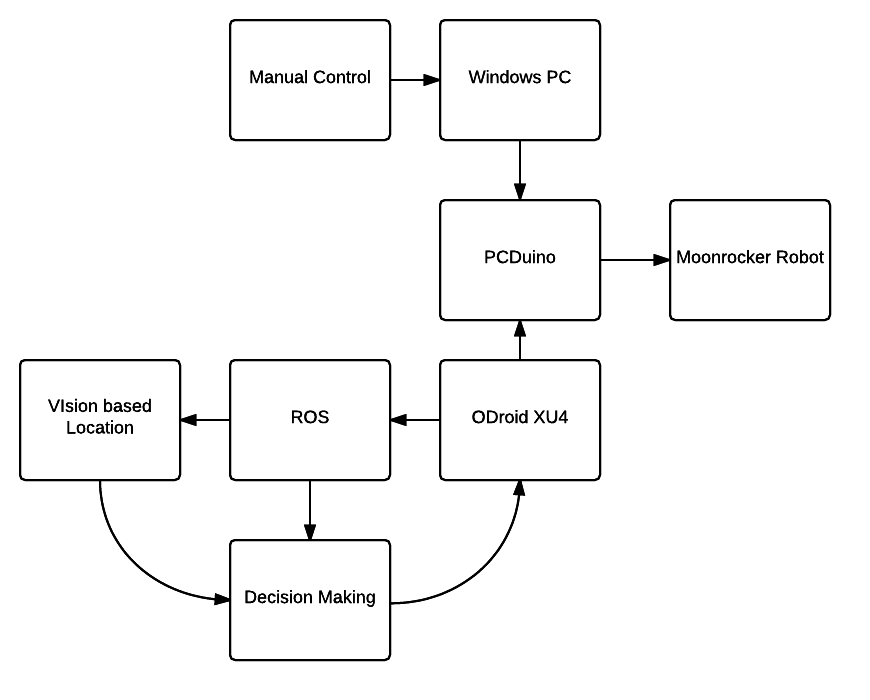
\includegraphics[width=0.75\textwidth]{./design}
\end{center}
\caption{System Diagram \label{systemdiagram}}
\end{figure}
\newpage
\section{Technologies Overview}
The technologies used to develop this system are the PCDuino, ODroid XU4, and ROS.
\vspace{2mm}

We chose to use the ODroid XU4 because it has 2 quad core processors which will be able to sufficiently handle the vision system, as well as the decision making system.
\vspace{2mm}


We chose to use ROS because it will help integrate the sensors in our system with the controls.
\vspace{2mm}


We chose to use the PCDuino because it was already integrated into our robotics system from the last year and currently runs out manual control systems.



